\documentclass[a4paper,11pt]{article}

% Packages
\usepackage[T1]{fontenc}
\usepackage[fontsize=11pt]{scrextend}
\usepackage[margin=2cm, bottom=2cm,right=2cm]{geometry}
\usepackage{amsmath}
\usepackage{amssymb}
\usepackage{parskip}
\usepackage{tabularx}
\usepackage{float}
\usepackage{booktabs}
\usepackage{mathtools}
\usepackage{latexsym}
\usepackage{enumitem}
\usepackage{lastpage}
\usepackage{multicol}
\usepackage{listings}
\usepackage{pdflscape}

% Use Helvetica font (comment out to default to Computer Modern)
\usepackage{helvet}
\renewcommand\familydefault{\sfdefault}
\allowdisplaybreaks

% Tikz
\usepackage{tikz}
\usetikzlibrary{arrows,shapes,calc,math,decorations.fractals,patterns,backgrounds,decorations.markings}
\tikzset{bluevec/.style={-triangle 45,blue,line width=1pt}}
\tikzset{convex/.style={draw,ellipse}}
\tikzset{point/.style={fill,circle,inner sep=1.5pt}}

% Title
\title{Rasterisation}
\author{Dr Jon Shiach}
\date{}

\begin{document}

\maketitle

\subsection*{Rasterising a line}

Fill in the pixels that are closest to the line joining the two points $(2,2)$ and $(11,7)$.

\begin{center}
    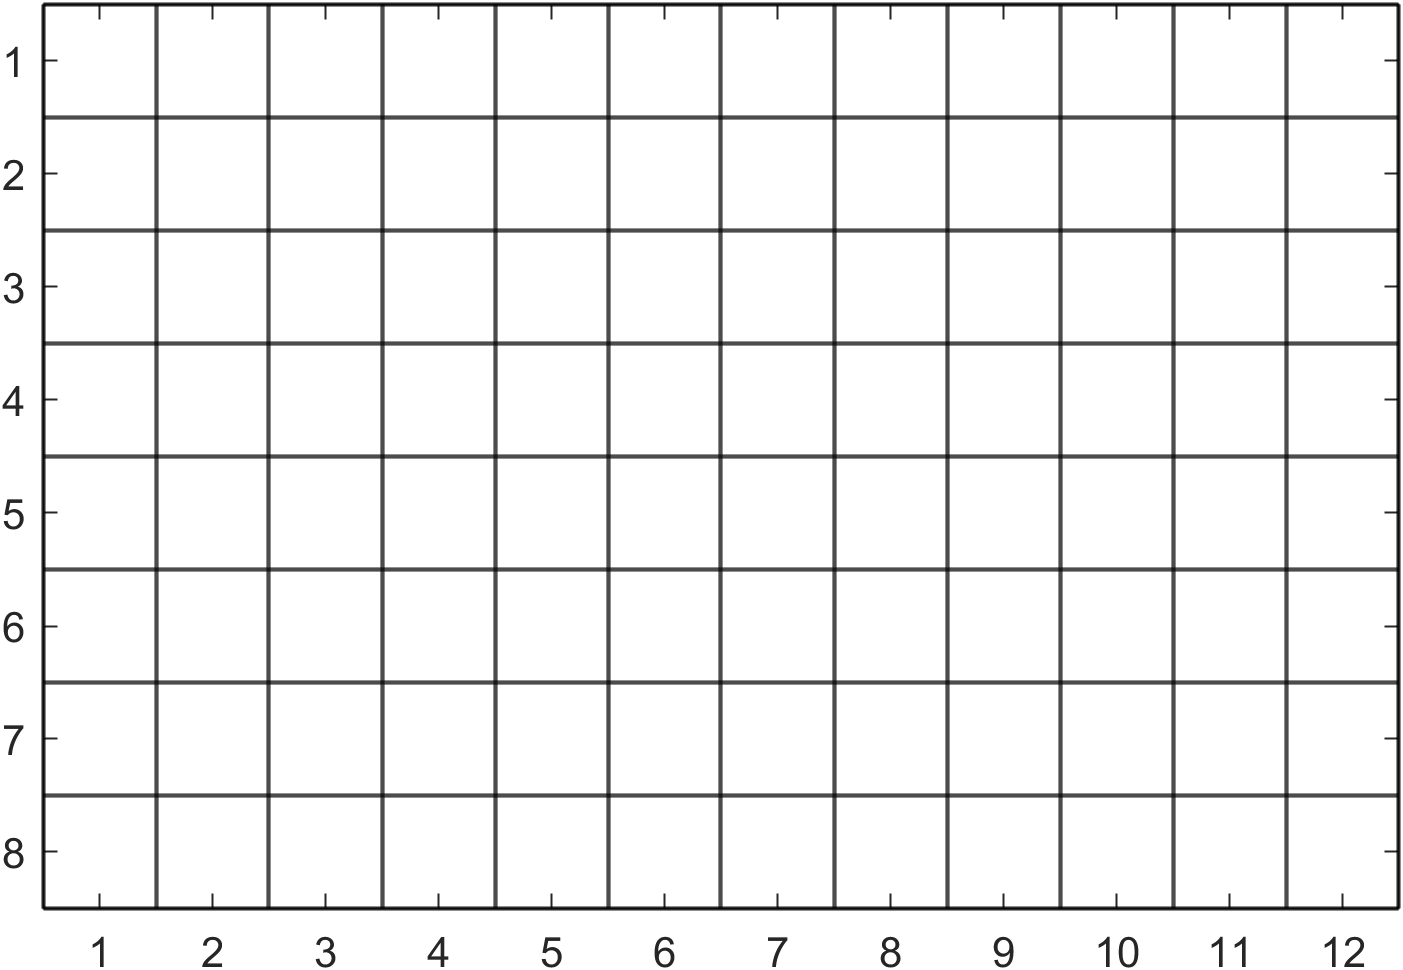
\includegraphics[width=6cm]{../images/12x8_grid.png}
\end{center}

\subsection*{Example 38}

Use the basic Bresenham's algorithm to determine the co-ordinates of the pixels on the straight line joining the two pixels with co-ordinates $(2, 2)$ and $(7, 5)$

\begin{center}
    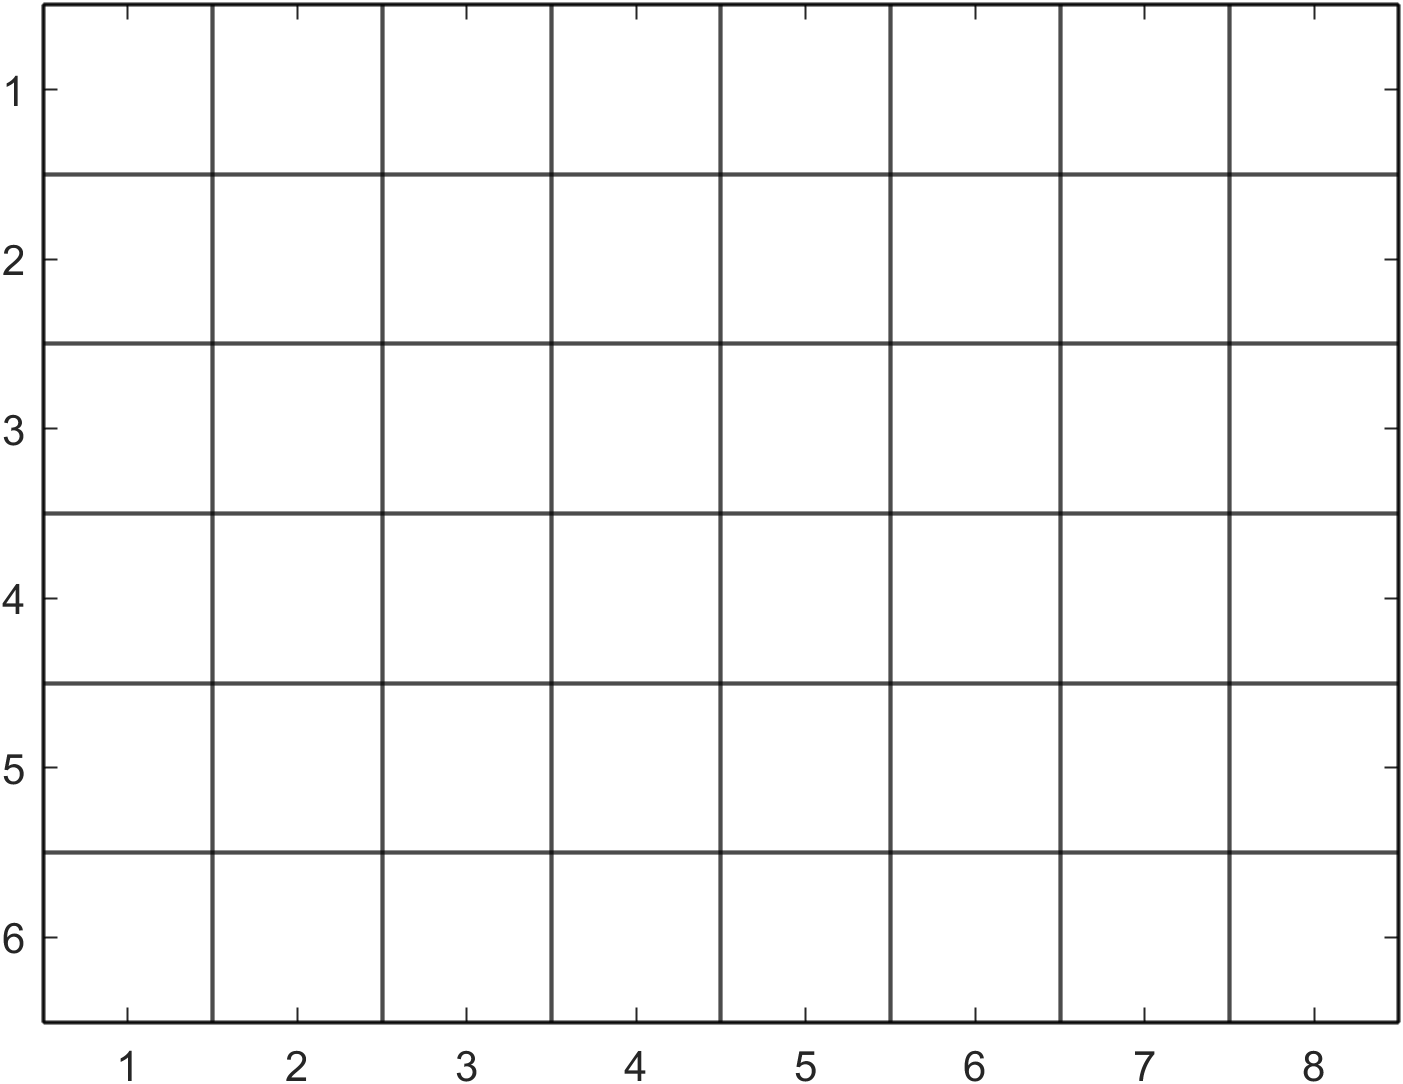
\includegraphics[width=4cm]{../images/8x6_grid.png}
\end{center}

\subsection*{Example 39}

Use Bresenham’s algorithm for drawing lines in any direction to determine the co-ordinates of
the pixels on the lines joining the following points:

\begin{enumerate}[label=(\roman*)]
    \item $(1,1)$ and $(5,7)$;
    \item $(7,2)$ and $(3,5)$.
\end{enumerate}

\begin{center}
    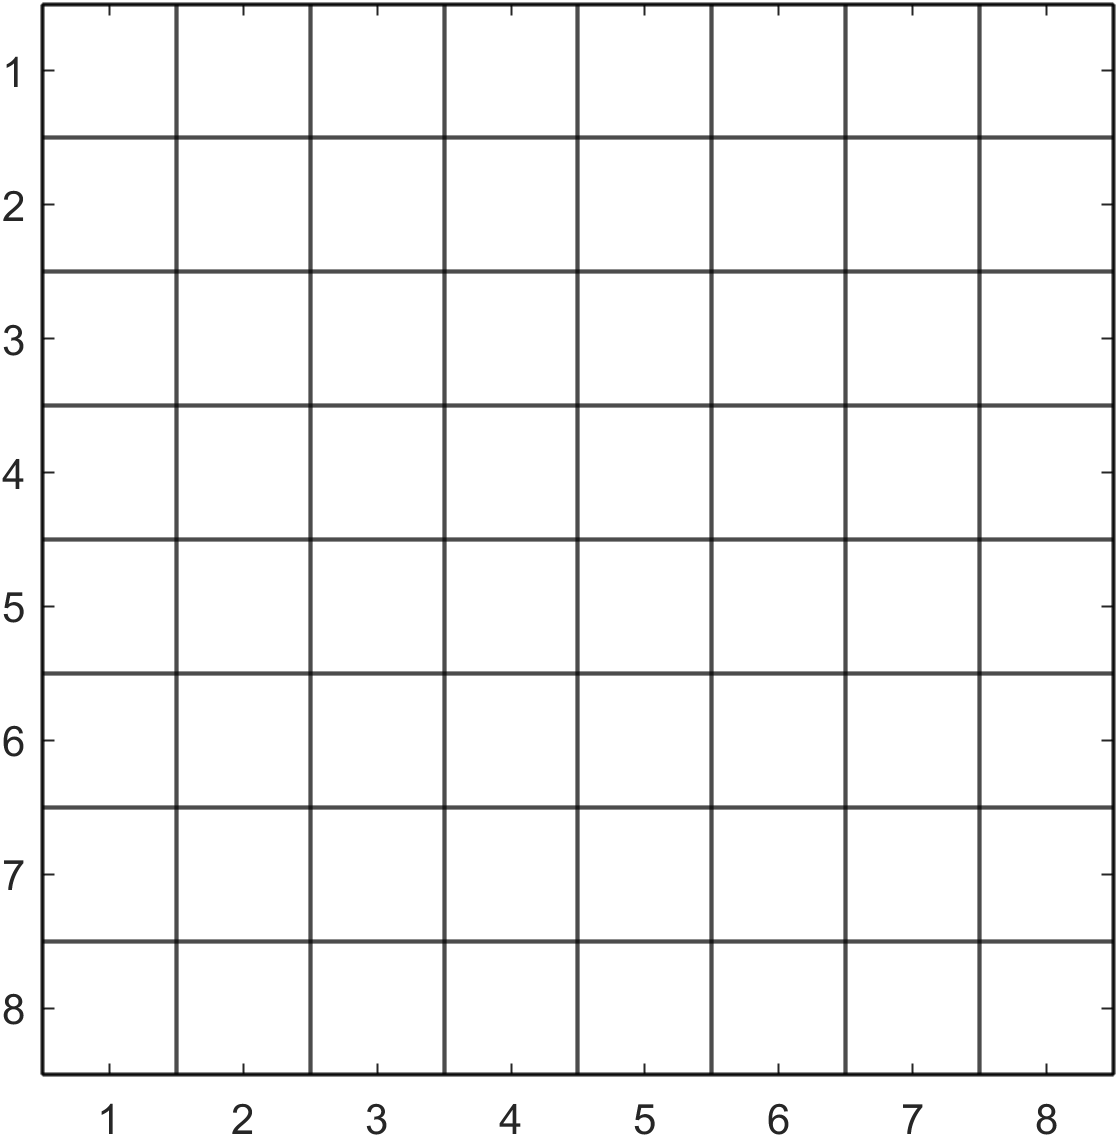
\includegraphics[width=4cm]{../images/8x8_grid.png}
    \hspace{2cm}
    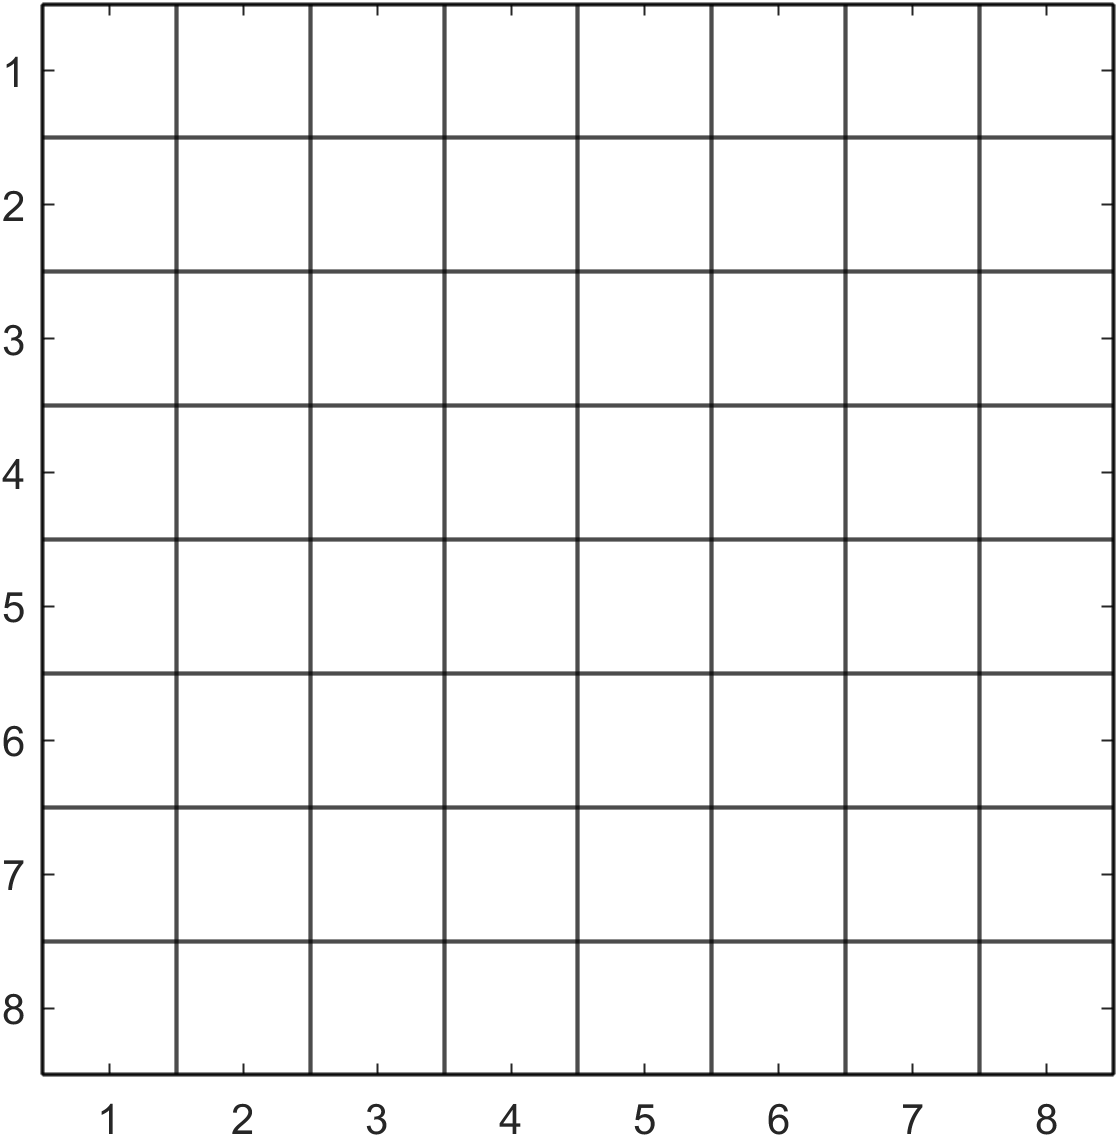
\includegraphics[width=4cm]{../images/8x8_grid.png}
\end{center}

\subsection*{Example 40} 

Use the midpoint algorithm to rasterise a circle centred at $(12, 12)$ with radius 10.

\begin{center}
    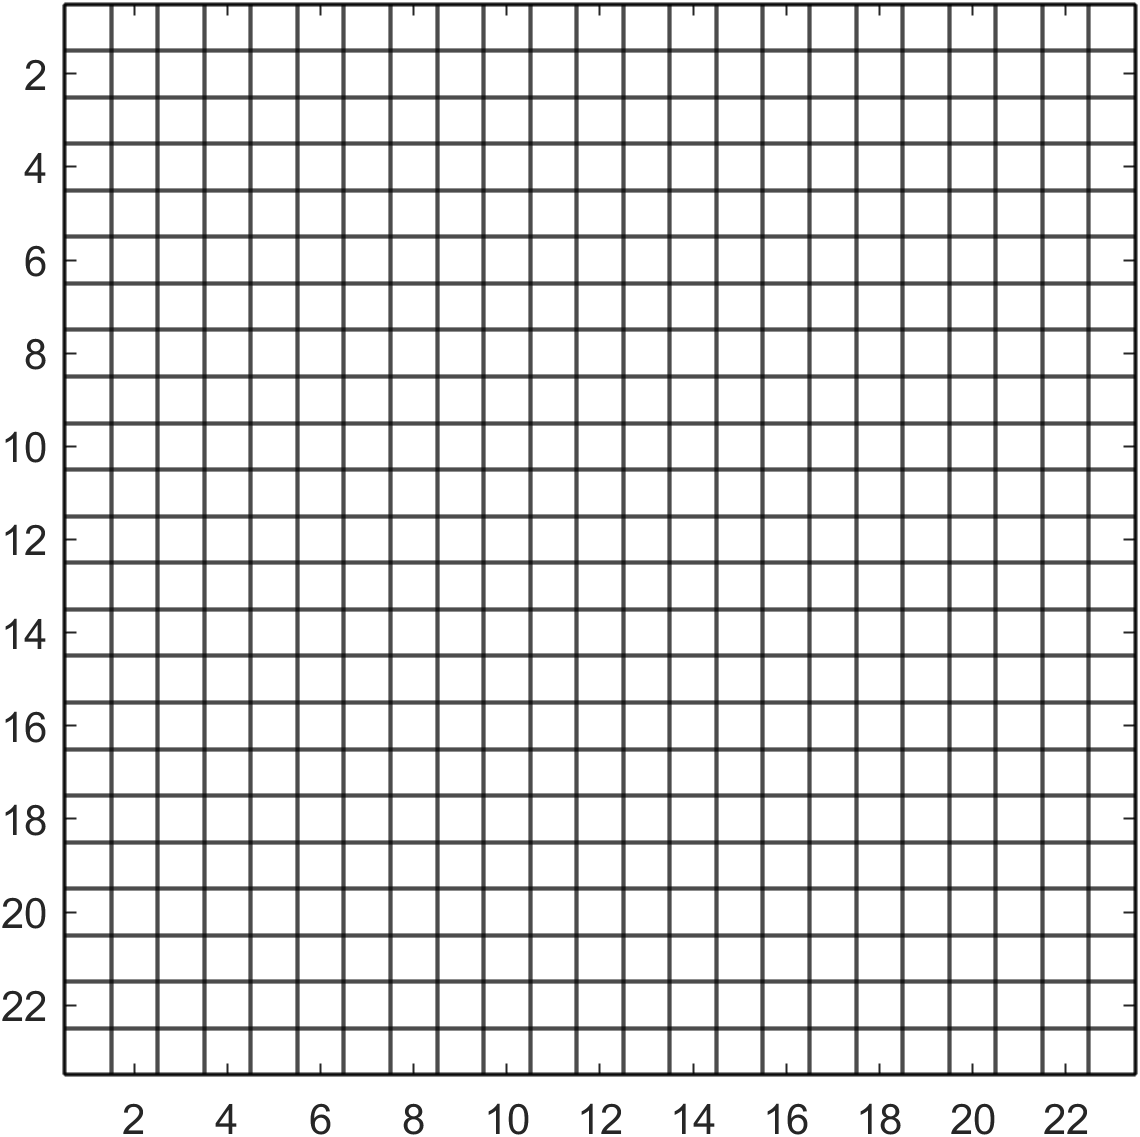
\includegraphics[width=8cm]{../images/23x23_grid.png}
\end{center}

\subsection*{Example 41}

Starting with the pixel at $(4, 4)$, use the flood fill algorithm to fill in the polygon on the raster below where the target colour is white and the replacement colour is blue.

\begin{center}
    \includegraphics*[width=4cm]{../images/flood_fill_example.pdf}
\end{center}

\subsection*{Example 42}

Use the scanline algorithm to draw the polygon defined below

\begin{center}
    \includegraphics*[width=7cm]{../images/scanline_example_0.png}
\end{center}


\end{document}